\documentclass[12pt]{article}
\usepackage{amsmath,graphicx,fullpage,float,setspace}
\begin{document}
\onehalfspacing
\begin{center}
	\textbf{Flattening the Curve}
\end{center}
	What follows is (I am sure) a standard exercise for a mathematical biology student. The model is simple:
\begin{equation}
	\text{Growth Rate of Infections} = \text{Contact Rate}\times\text{Fraction of Population Infectable}
\end{equation}
By ``contact rate'' I simply mean the number of people one might contact during a certain period of time. Ignoring immunity, we might imagine that the contact rate is two, in which case the number of infected people would double. Considering immunity, we conclude that a fraction of those with which one comes into contact have already been infected and are therefore immune. Early on, the contact rate determines the growth rate of infections, but as more people become infected, there are fewer people to infect , and so the growth rate of infection falls, giving us the now iconic curve which we are to ``flatten'' (see the Figure below). 

\begin{figure}[H]
	\begin{center}
		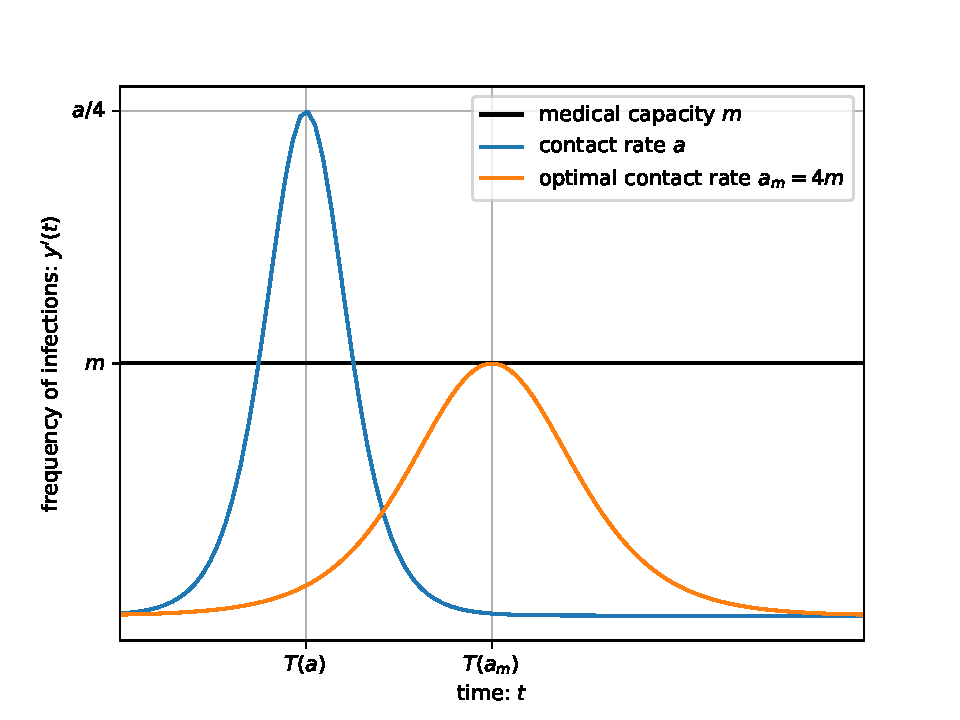
\includegraphics{curve}
	\end{center}
\end{figure}

While the intuition is sound, we haven't done any math yet (a shame!) and it is not yet clear by how much we should lower the contact rate (that is to say, how much social-distancing we should practice) to prevent hospitals from overflowing. Formally, for each time $t\geq0$, let $y(t)\in[0,1]$ denote the fraction of the population that has been infected by time $t$ (and are therefore immune). Let $y_{0}=y(0)$. Finally, let $a>0$ denote our so-called contact rate. $y$ evolves according to
\begin{equation}\label{equation:main}
	\frac{dy}{y}=(a\: dt)(1-y). 
\end{equation}
Over an interval of time of length $dt$, the growth rate in the fraction of the population that is infected, $dy/y$, equals the fraction of the population with which one might contact during the the interval of time, $a\: dt$, times the fraction of the population that has already been infected (and is therefore immune). An important assumption lurks in the background: someone who becomes infected at time $t$ is sick only during $[t,t+dt)$ and then immediately becomes immune. Rearranging Equation \ref{equation:main}, we obtain the Bernoulli differential equation 
\begin{equation}
	y'(t)=ay(t)(1-y(t))
\end{equation} 
which can be integrated in closed form (although it is not necessary, and although it is not necessary, I will integrate it nonetheless as it is a Bernoulli differential equation, which is one of personal favorites):
\begin{equation}
	y(t)=\frac{y_{0}\exp(at)}{y_{0}\exp(at)+(1-y_{0})}
\end{equation}
Lovely. Now time for some analysis. $y'$ attains its maximum of $a/4$ at time $t=T(A)$, where
\begin{equation}
	T(a)\equiv\frac{1}{a}\log\left(\frac{1-y_{0}}{y_{0}}\right)
\end{equation}
Suppose that the medical system has a capacity of $m>0$ (where $m$ can be interpreted as the number of available beds during $[t,t+dt)$). To find the ``optimal'' contact rate $a$ for which the number of infected over $[t,t+dt)$ never exceeds $m_{0}$:
\begin{equation}
	a_{m_{0}}=4m_{0}.
\end{equation}
In a richer model, one might account for encubation time, state-dependent contact rates, changes in medical capacity, uncertainty, etc. Alas, I am a humble economist with nothing much to offer in this direction. The hour grows late and my co-authors' patience grows thin.
\end{document}
